\chapter{彩虹表算法的实现}
\section{彩虹表的算法分析}
\label{sec:3.3}
	\subsection{非完美彩虹表}
如\ref{sec:3.1}节所述,Hellman表的一个主要不足是表大小的限制,当以增大表大小来获得更高得成功率时,表中的节点碰撞而导致的链合并概率也会随之增加,且增加的比例同m与t的平方成正比。为了解决这一不足,在2003年,Oechslin在Hellman算法的基础上结合了Rivest的差异点(DP)的优势,提出了一种在当时比较先进的算法--彩虹表算法\cite{PO}。通过这种时空折中算法预运算所生成的表,我们称之为彩虹表(Rainbow Table),彩虹表中的行称为彩虹链。
与Hellman算法在一张表中只使用一个f函数不同,彩虹表的每一列使用的R函数都不一样,以构造不同的f函数,如式\eqref{equ:3.10}所示:
\begin{equation}
\label{equ:3.10}
f_i(k)=R_i(S_k(P)) \quad \quad  (1\leq i \leq t) 
\end{equation}
从上式可以看出,彩虹表用$R_1,R_2,\ldots ,R_t$代替Hellman表中的R函数。因此,只有在当彩虹表中两个节点在同一列发生碰撞时,才会发生链合并。换句话说,如果碰撞发生在不同列的两个节点,由于不同列采用的不同的R函数,碰撞点之后的链不会被合并。
我们假设一张彩虹表有m条彩虹链,每条彩虹链的长度为t,即为$m\times t$的矩阵,如式\eqref{equ:3.11}:
\begin{equation}
\label{equ:3.11}
\begin{bmatrix}
k_{1,1} & k_{1,2} & \cdots & k_{1,t-1} & k_{1,t} \\
k_{2,1} & k_{2,2} & \cdots & k_{2,t-1} & k_{2,t} \\
\vdots & \vdots & \vdots & \vdots & \vdots \\
k_{m,1} & k_{m,2} & \cdots & k_{m,t-1} & k_{m,t} \\
\end{bmatrix}
\end{equation}
现在来计算这张彩虹表的破解成功率P,这个问题实质上等价与整个矩阵每列的概率乘积。第一个元素$k_{1,1}$命中的概率为$\frac{1}{N}$,那么这一列命中概率为$P_1=\frac{m_{1}}{N}$;则第二列命中的概率为$P_2=1-(1-\frac{1}{N})^{m_1}$,当$N\gg m_{1}$时,$P_2=1-e^{-\tfrac{m_1}N{}}$,因此,可以得到第i列的命中概率公式:
\begin{equation}
P_i=1-e^{-\tfrac{m_{i-1}}{N}}=\frac{m_i}{N}
\end{equation}
在概率定理可以推出整张彩虹表的成功率公式为:
\begin{eqnarray}
\label{equ:3.12}
P_{Rainbow} \ge 1-\prod^{t}_{i=1}\left(1-\frac{m_{i}}{N}\right) \nonumber\\
\text{其中,} m_{1}=m \text{,且} m_{n+1} = N\left(1-e^{-\tfrac{m_{n}}{N}}\right)
\end{eqnarray}

比较\eqref{equ:3.7}式和\eqref{equ:3.12}式,我们可以发现t张$m\times t$Hellman表与1张$mt\times t$的彩虹表有大致相同的成功率。因为这两种算法所产生的表都覆盖了$mt^2$的密钥空间,同时也都包含了t个不同的R函数。在假警方面,两者也有类似的共同点,单张彩虹表的一列以及t张Hellman表,若包含mt个节点,则这些节点中的任一碰撞都将会导致链的合并。
上述这样等规模的Hellman表和彩虹表的比较可以参考式\eqref{equ:3.20}
\begin{gather}
\label{equ:3.20}
\begin{bmatrix}
k_{1,0}^1\xlongrightarrow{f_1} k_{1,1}^1\xlongrightarrow{f_1} \cdots \xlongrightarrow{f_1}k_{1,t}^1 \\
\vdots \\
k_{m,0}^1\xlongrightarrow{f_1} k_{m,1}^1\xlongrightarrow{f_1} \cdots \xlongrightarrow{f_1}k_{m,t}^1 \\
\end{bmatrix} \\ 
\begin{bmatrix}
k_{1,0}^t\xlongrightarrow{f_t} k_{1,1}^t\xlongrightarrow{f_t} \cdots \xlongrightarrow{f_t}k_{1,t}^t \\
\vdots \\
k_{m,0}^t\xlongrightarrow{f_t} k_{m,1}^t\xlongrightarrow{f_t} \cdots \xlongrightarrow{f_t}k_{m,t}^t \\
\end{bmatrix}\\
\begin{bmatrix}
k_{1,0}^1\xlongrightarrow{f_1} k_{1,1}^1\xlongrightarrow{f_2} \cdots \xlongrightarrow{f_t}k_{1,t}^1 \\
k_{2,0}^1\xlongrightarrow{f_1} k_{1,1}^1\xlongrightarrow{f_2} \cdots \xlongrightarrow{f_t}k_{2,t}^1 \\
\cdots \\ 
\\ \\
\cdots \\
k_{mt-1,0}^1\xlongrightarrow{f_1} k_{1,1}^1\xlongrightarrow{f_2} \cdots \xlongrightarrow{f_t}k_{mt-1,t}^1 \\
k_{mt,0}^1\xlongrightarrow{f_1} k_{1,1}^1\xlongrightarrow{f_2} \cdots \xlongrightarrow{f_t}k_{mt,t}^1
\end{bmatrix}
\end{gather}
在线分析过程中,彩虹表算法的搜索过程与Hellman算法有所不同,首先,将给定的密文C代入$R_t$的$y_1$,并检索是否存在某个$EP_i=y_1$,如果找到了匹配的$EP_i$,这可以通过保存的对应$SP_i$来恢复$k_{t,t-1}$。若找不到匹配的EP,则将密文C依次代入$R_{t-1}$,再次搜索判断是否存在正确的密钥在第t-2列中。以此类推,最坏的情况下将遍历表中所有的t列,以f函数迭代次数为标准,这个代价为$1+2+\cdots +(t-1)=\frac{t(t-1)}{2}$次。而Hellman表需要搜索$t^2$次,因而单张的彩虹表相比t张Hellman表,搜索代价只有不到Hellman算法的一半。

在此小结一下彩虹表相对Hellman表的优点:\\
1),从搜索次数角度来看,彩虹表最多需要比较$log(mt)*t$次,而Hellman表将最多需要$log(t)*t^2$,即搜索t表t列。因此彩虹表的比较次数约为Hellman的$\frac{1}{t}$,彩虹表相应的TMTO曲线为:
\begin{equation}
TM^2=\frac{1}{2}N^2
\end{equation}
2),彩虹表中若发生彩虹链合并时,则会导致对应的EP点相同。当需要构造没有重复链的完美表(Perfect Table)时,可以通过检查EPs来完成。而Hellman表则无此特性。需要注意的是在完美表中并不是没有碰撞节点,而是碰撞节点不在同一列上出现。\\
3),由于彩虹链中的t个R函数均不相同,因此链中将几乎不会产生循环。以Hellman链为例,若同一链中出现了两个节点$k_i,k_j$,使得$k_i=k_j$,那么由于该链使用相同的R函数,故从这两个相同节点的后面节点都会相等,依次类推,最多会导致j-i个节点的重复,进而缩小了整个Hellman表的覆盖率。该现象不会产生假警,然而会降低成功率。而彩虹表则没有相应的问题。\\
4),与Hellman表的变形差异点(DP)算法相比,彩虹表的链条长度是固定的,这个特性对彩虹表的程序代码实现是十分有利的,同时也会使得假警率有所下降,从而提高了成功率。
	\subsection{完美彩虹表}
当表中出现合并链时,彩虹表和差异点DP算法都可以通过检查是否具有相同的EP节点方式来检测出合并,而通常情况在预运算后生成的表需要排序的,这样一来就可以很容易地从表中剔除重复的链,而经过剔除重复链后的表我们称之为完美彩虹表。特别是在当内存空间有限时,我们总希望表能包含尽可能多的唯一节点,以提高成功率。生成相对应的Hellman完美表,则不得不搜索整张表,每个节点均要O(mt)次搜索,显然这是不现实的。在完美彩虹表中,有$m_i=m_1=m (2\leq i \leq t)$,因此成功率可化简为:
\begin{equation}
\label{equ:3.13}
P_{perfect}=1-\prod^{t}_{i=1}\left(1-\frac{m}{N}\right)
\end{equation}

从\eqref{equ:3.13}式可知,成功率直接与完美彩虹表的初始参数m,t有关,也就是表越大,成功率$P_{perfect}$应越大。同时与非完美彩虹表比较,不但减少了因存储重复节点而造成的空间浪费,而且节省了在线分析的时间代价。对于一个给定的t,假设选择$m_1=N$时得到的$m_t \text 为 m_{max}(t)$,表示为完美彩虹表最大的独立结束节点EPs的个数,其中$m_{i+1}=N\left(1-e^{-\tfrac{m_i}{N}}\right)(1\leq i \leq t)$。

当$t\gg 1$时,利用泰勒公式可以得到\cite{aa}:
\begin{equation}
m_{max}(t)\approx \dfrac{2N}{t+2}
\end{equation}
将上式代入\eqref{equ:3.13}式便可得出完美彩虹表成功率的最大期望值为:
\begin{equation}
P_{perfect}^{max}=1-\left(1-\dfrac{m_{max}}{N}\right)^t \approx 1-e^{-t\tfrac{m_{max}}{N}} \approx 1-e^{-2} \approx 86\%
\end{equation}
也就是说,对于N和较大的t,完美彩虹表的成功率会随着m,t的增大而趋于一个常量。因此,单张的彩虹表的成功率要小于80\%,若要较高的成功率P$(P>90\%)$,则可以通过多张彩虹表来实现。

\section{彩虹表的构建与产生}
\subsection{密钥的生成}
首先用随机函数生成一个Index,为了确保Index在密钥空间N里,我们对Index进行取模运算:$Index\quad mod \quad N$。再执行IndexToPlain()函数得到在初始设定的密钥空间N里的密钥。
\subsection{定义Hash函数}
本文的实现了对SHA-1、MD5和LM三种Hash函数的破解,下面代码对LM算法的实现:
\begin{lstlisting}
void HashLM(unsigned char* pPlain, int nPlainLen, unsigned char* pHash)
{   
  int i; 
  for (i = nPlainLen; i < 7; i++)
  pPlain[i] = 0;
  static unsigned char magic[] = {0x4B, 0x47, 0x53, 0x21, 0x40, 0x23, 
                                                            0x24, 0x25};
  des_key_schedule ks;
  setup_des_key(pPlain, ks);
  des_ecb_encrypt((des_cblock*)magic,(des_cblock*)pHash,ks,DES_ENCRYPT);
}
\end{lstlisting}
SHA1和MD5函数的实现则是调用了OpenSSL的API函数:
\begin{lstlisting}
unsigned char *MD5(const unsigned char *d, size_t n, unsigned char *md);
\end{lstlisting}
\begin{lstlisting}
unsigned char *SHA1(const unsigned char *d, size_t n, unsigned char *md);
\end{lstlisting}
\subsection{定义Reduce函数}
Reduce函数是将密文映射到密钥空间中,彩虹链中的每个位置使用的Reduce函数都是不同的,因此我们可以将彩虹链的位置作为Reduce函数的主要参数进行计算。所以Reduce函数定义如下:
\begin{equation}
R(\text{密文},\text{密钥})=(\text{密文+链位置+偏移量})\quad mod \quad \text{密钥总空间}
\end{equation}
具体的代码实现如下:
\begin{lstlisting}
void CChainWalkContext::HashToIndex(int nPos)
{
  m_nIndex = (*(uint64*)m_Hash + m_nReduceOffset + nPos)
                                   % m_nPlainSpaceTotal;
}

\end{lstlisting}
\subsection{彩虹表参数}
彩虹表算法中几乎每个参数都对构建一个高质量的彩虹表有影响,比如参数m决定彩虹表存储空间大小,t决定在线分析的时间,彩虹表张数l代表了彩虹表的存储个数,同时也影响着破解成功概率。如何有机地组合这些参数构成最优的
\subsection{构建彩虹表}
彩虹表算法实现的首要事情就是要产生符合自己需求的彩虹表文件,本次实现要求彩虹表的破解成功率在99.9%以上。

彩虹表算法中有许多参数变量,在构造一张彩虹表前必须先弄明白每个参数的含义,在这里我们为了方便下文叙述,统一给出彩虹表算法中会出现的参数和变量:Hash计算能力,取决于CPU和GPU等硬件设备;硬盘读写速度,取决于硬盘;密钥空间N;
\begin{enumerate}
\item 每条彩虹链的长度t;
\item 一张彩虹表中彩虹链的个数m;
\item 彩虹表的个数L;
\item 磁盘占用量M\quad 彩虹表所占用的存储空间;
\item 破解成功率P\quad 破解密钥的成功概率;
\item 破解时间;
\item 预运算时间;
\end{enumerate}
由上述可知,一张彩虹表是由许多彩虹链组成的,每个彩虹链在程序中的数据结构如下:\\
\begin{lstlisting}
struct RainbowChain 
{
	unit64 nIndexS;		//链表的初始元素
	unit64 nIndexE;		//链表的末尾元素
}
\end{lstlisting}
函数主要输入参数:
\begin{lstlisting}
	string sHashRoutineName  = argv[1];	
	//需要破解的算法名称
	string sCharsetName      = argv[2];				
	int nPlainLenMin         = atoi(argv[3]);
	//密码长度最小值
	int nPlainLenMax         = atoi(argv[4]);
	//密码长度最大值
	int nRainbowTableIndex   = atoi(argv[5]);			
	int nRainbowChainLen     = atoi(argv[6]);			
	int nRainbowChainCount   = atoi(argv[7]);			
\end{lstlisting}
生成彩虹表的关键代码:
\begin{lstlisting}
	int i;
	for (i = nDataLen / 16; i < nRainbowChainCount; i++) 
	{
		cwc.GenerateRandomIndex();
		uint64 nIndex = cwc.GetIndex();
		int nPos;
		for (nPos = 0; nPos < nRainbowChainLen - 1; nPos++)
		{
			cwc.IndexToPlain();
			cwc.PlainToHash();
			cwc.HashToIndex(nPos);		//缩减函数
		}
		nIndex = cwc.GetIndex();

\end{lstlisting}

初始节点nIndexS由cwc.GenerateRandomIndex()函数随机产生,并把当前的index值也赋予CChainWalkContext.m\_nIndex中, m\_nindex起到中间记录作用,当经过nRainbowChainLen(参数t)次循环计算得到nIndexE。

彩虹表生成算法描述:
\begin{enumerate}
\item 将随机生成的nIndexS通过函数cwc.IndexToPlain()转化成明文Plain,这一转化过程与二进制转16进制差不多,只是根据明文字符集长度(m\_nPlainCharsetLen)来变化;
\item 对步骤1生成的Plain进行Hash函数计算,通过PlainToHash()函数实现;
\item 对步骤2生成的Hash值进行缩减运算,缩减函数为HashToIndex(nPos),最后得到的nIndex必须在预设的字符空间范围内。
\end{enumerate}

将以上三步循环nRainBowChainLen次数后,我们将得到nIndexE和彩虹链的长度,当生成了m条彩虹链之后,这些彩虹链所组合起来的就是一张彩虹表文件。由于在循环过程中所产生的index只保存在内存里,并不写入磁盘文件,但是我们依然可以通过初始的Index计算出这过程中所有的index值。
\begin{equation}
\label{equ:4.1}
\begin{bmatrix}
Index\_Start_1 & Index\_End_1 \\
Index\_Start_2 & Index\_End_2 \\
\vdots  & \vdots \\
Index\_Start_m & Index\_End_m 
\end{bmatrix}
\end{equation}
从彩虹表的结构\eqref{equ:4.1}我们可以很容易得知一个彩虹链的所占的磁盘空间为$2*64=128$比特,也就是16Byte。由此得到彩虹表磁盘空间占用公式:
\begin{equation}
\label{equ:4.2}
M=16*m*l
\end{equation}
其中m为彩虹链的条数,l为彩虹表的个数。图\ref{fig:4.1}为彩虹表生成程序,hash\_algorithm 为目标密码hash算法;charset为密钥的字符集,决定这张彩虹表的密钥空间;还有链表长度和链表个数等参数。
\begin{figure}[!ht]
\centering
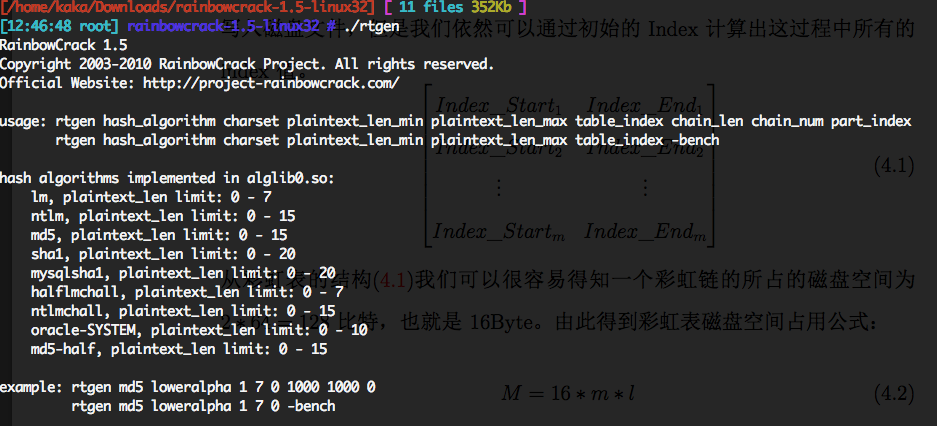
\includegraphics[scale=0.4]{4-1.png}
\caption{彩虹表生成程序}
\label{fig:4.1}
\end{figure}
\begin{figure}[!ht]
\centering
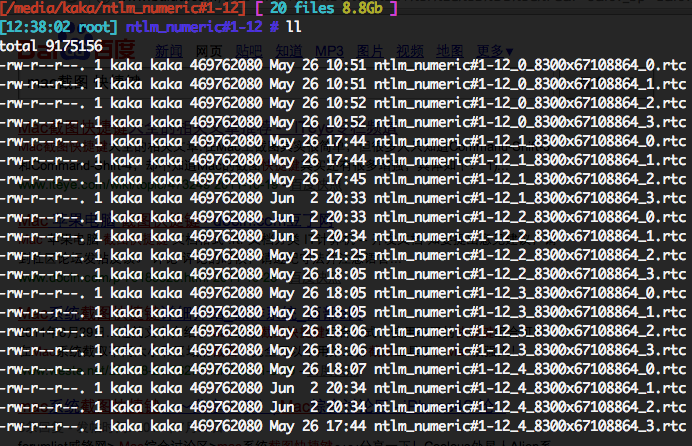
\includegraphics[scale=0.5]{4-2.png}
\caption{ntlm算法彩虹表}
\label{fig:4.2}
\end{figure}
从图\ref{fig:4.2}中我们可以看到20张彩虹表,hash\_algorithm为ntlm算法,ntlm为Windows NT系统的用户登陆验证算法;密钥字符集为numeric,也就是0~9,最小长度为1,最大长度为12,因此这个密钥空间$N=10^{12}+10^{11}+ \cdots +10^2 +10$,其他的密钥并不在这20张表里,一定不会被搜索到,想要破解需要加大链的数目,或者链表长度,或者表的张数;链表长度为8300,链表个数为67108864,这样通过公式\eqref{equ:4.2}我们很容易到这20张表的所占用的磁盘空间$M=20GB$,每张表的大小为1GB。
\section{密钥破解}
\subsection{搜索算法}
用彩虹表进行破解的过程其实质就是对彩虹表文件进行整表搜索的过程,简单来讲就是查表。破解的成功率和破解的时间基本上由预运算所生成的彩虹表决定,生成优质的彩虹表对破解的效率影响很大。具体的优化方法和技巧我们将在下文详细介绍,这一节我们要讨论的是彩虹表如果进行查表破解。首先我们看图\ref{fig:4.3}:
\begin{figure}[!ht]
\centering
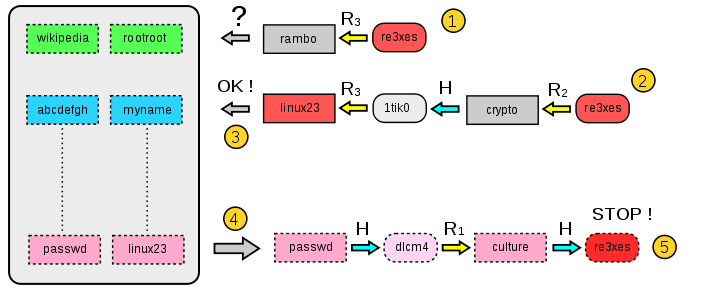
\includegraphics[scale=0.5]{crack}
\caption{彩虹表查表过程}
\label{fig:4.3}
\end{figure}

从图中我们看到需要破解的密钥为“re3xes”,第一步,将“re3xes”代入R函数,得到索引“rambo”,将此索引从每个彩虹链的末端开始对比;
第二步,若不匹配,则通过算法中的f函数\eqref{equ:3.10}进行遍历整条彩虹链,若在这条链表中没找到匹配的,则往后遍历表中的其他彩虹链;
第三步,当在链中找到匹配的索引后,记录该链表的首部索引;
第四步,通过第三步找到的索引,进行f函数计算得到产生目标密钥“re3xes”的明文“passwd”,并验证其正确性。
\subsection{假警分析}
无论是上一章介绍的Hellman经典算法,还是本文采用的彩虹表算法,都是会发生假警,假警的最大弊端是对存储资源和计算时间造成严重的重复和浪费,因此对假警的检测尤为重要,彩虹表算法中采用的检查点技术用于检测假警,通过实验表明,增加0.89\%的内存用于存储检查点节省了10.99\%的密码分析时间。
\section{实验结果与分析}

\section{本章小结}
本章主要介绍了彩虹表算法的C++实现,主要包括彩虹表的预运算,即彩虹表的生成和利用彩虹表进行密钥破解。关键的程序代码可以参考附件。
